\documentclass[addpoints]{exam}
\usepackage[utf8]{inputenc}
\usepackage[spanish]{babel}
\usepackage[T1]{fontenc}
\usepackage{charter}
\usepackage{amsmath}
\usepackage{amsfonts}
\usepackage{amssymb}
\usepackage{graphicx}
\usepackage{tikz}
\usepackage[outline]{contour} % glow around text
\usetikzlibrary{babel,calc,patterns,decorations.pathmorphing,decorations.markings,arrows.meta,shapes.geometric}
\usetikzlibrary{calc}
\tikzset{>=latex}
\contourlength{1.1pt}
\usepackage{tikz-3dplot}
\usepackage{multicol}
\usepackage{exam-randomizechoices}
\usepackage[left=1cm,right=1cm,top=2cm,bottom=2cm]{geometry}
\usepackage[font=small,labelfont={small,bf},margin=0.5cm,justification=justified]{caption}
\usepackage[font=small,labelfont={small,bf}]{subcaption}
\usepackage[italic,defaultmathsizes]{mathastext}
\usepackage{hyperref}
\usepackage{calculator}
\usepackage[breakable]{tcolorbox}
\usepackage{multirow}
\usepackage{tabularx}
\usepackage{cancel}
\usepackage{tipa}
\usepackage{enumerate}

%\pointpoints{punto}{puntos}
%\bonuspointpoints{punto extra}{puntos extra}

\renewcommand{\solutiontitle}{\textbf{Solución: }}
\renewcommand{\thequestion}{\bfseries\arabic{question}}

\newcommand{\sgn}{\mathop{\mathrm{sgn}}}
\newcommand{\diff}[0]{\mathrm{d}}
\newcommand{\fdiff}[2]{\frac{\mathrm{d} #1}{\mathrm{d} #2}}
\newcommand{\pdiff}[2]{\frac{\partial #1}{\partial #2}}
\newcommand{\fddiff}[2]{\frac{\mathrm{d^2} #1}{\mathrm{d} #2^2}}
\newcommand{\pddiff}[2]{\frac{\partial^2 #1}{\partial {#2}^2}}
\newcommand{\grado}[0]{^{\circ}}
\newcommand{\angulo}[3]{#1\grado \, #2' \, #3''}
\newcommand{\chel}[4]{^{#1}_{#2}\mbox{#3}^{#4}}
\newcommand{\valmed}[1]{\left\langle #1 \right\rangle}
\newcommand{\E}[1]{\times 10^{#1}}
\newcommand{\ver}[1]{\hat{\mathbf{#1}}}
\newcommand{\vecg}[1]{\boldsymbol{#1}}
\newcommand{\iu}{\mathrm{i}}
\newcommand{\norm}[1]{\left\vert\left\vert #1 \right\vert\right\vert}
\newcommand{\abs}[1]{\left\vert #1 \right\vert}
\newcommand{\tens}[1]{\mathbb{#1}}
\newcommand{\rr}{\mathbb{R}}
\newcommand{\un}[1]{\text{#1}}
\newcommand{\logoUNAHUR}{
\includegraphics[scale=0.35]{/home/shluna/Proyectos/Clases_Fisica_III/imgs/logo_unahur.png }}
\renewcommand{\arraystretch}{1.5}
\newcommand{\rta}{\textbf{Respuesta: }}
\newcommand{\rtas}{\textbf{Respuestas: }}
\newcommand{\ang}{110}
\newcommand{\angu}{-30}
\newcommand{\rad}{4}
\newcommand{\mg}{1}
\newcommand{\muc}{0.5}
\newcommand{\arc}[1]{{%
  \setbox9=\hbox{#1}%
  \ooalign{\resizebox{\wd9}{\height}{\texttoptiebar{\phantom{A}}}\cr#1}}}

  \colorlet{mydarkblue}{blue!40!black}
  \colorlet{myblue}{blue!30}
  \colorlet{myred}{red!65!black}
  \colorlet{vcol}{green!45!black}
  \colorlet{watercol}{blue!80!cyan!10!white}
  \colorlet{darkwatercol}{blue!80!cyan!80!black!30!white}
  \tikzstyle{water}=[draw=mydarkblue,top color=watercol!90,bottom color=watercol!90!black,middle color=watercol!50,shading angle=0]
  \tikzstyle{horizontal water}=[water,
    top color=watercol!90!black!90,bottom color=watercol!90!black!90,middle color=watercol!80,shading angle=0]
  \tikzstyle{dark water}=[draw=blue!20!black,top color=darkwatercol,bottom color=darkwatercol!80!black,middle color=darkwatercol!40,shading angle=0]
  \tikzstyle{vvec}=[->,very thick,vcol,line cap=round]
  \tikzstyle{force}=[->,myred,very thick,line cap=round]
  \tikzstyle{width}=[{Latex[length=3,width=3]}-{Latex[length=3,width=3]}]

\hypersetup{
%      draft,
   linktocpage=true,
    colorlinks=true,
    linkcolor=blue,
    citecolor=blue,
    filecolor=blue,      
    urlcolor=blue
}

\printanswers
\qformat{\textbf{Ejercicio \thequestion}\hfill}

\pagestyle{headandfoot}
\firstpageheader{Instituto de Tecnología e Ingeniería}{\logoUNAHUR}{Física III}
\firstpageheadrule
\runningheader{Examen integrador y final}{\logoUNAHUR}{Física III}
\runningheadrule
\firstpagefooter{}{Página \thepage\ de \numpages}{}
\firstpagefootrule
\runningfooter{}{Página \thepage\ de \numpages}{}
\runningfootrule

\begin{document}

\renewcommand{\tablename}{Tabla}

\tdplotsetmaincoords{70}{110}

\begin{tcolorbox}[colback=white,arc=0mm,colframe=black]
    \begin{center}
        \Large\textbf{Física III -- Examen integrador y final}
    \end{center}
\end{tcolorbox}

\begin{itemize}
    \item \makebox[0.75\textwidth]{Nombre y apellido:\enspace\hrulefill}
    \item \makebox[0.75\textwidth]{DNI:\enspace\hrulefill}
\end{itemize}

\begin{questions}

    \question Un resorte de constante $k_1$ se une a un bloque de masa $m$. Luego el sistema formado por estos se dispone en dirección horizontal y se lo hace oscilar alrededor de la posición de equilibrio del resorte. Si se observa que el periodo es $P_1$, mostrar que si el resorte se reemplaza por otro de constante $k_2$, el sistema formado por este nuevo resorte y el bloque oscilará con un periodo $P_2$ dado por: $$ P_2 = P_1 \sqrt{\frac{k_1}{k_2}}.$$
    
    \question \label{ej:volante_hueco} Un volante, que tiene forma de un cilindro hueco, de masa $M$, radio interno $R_0$ y radio externo $R$, puede girar alrededor de un eje horizontal que pasa por su centro geométrico, el cual se indica con el punto $O$ de la Figura~\ref{fig:volante_hueco}. Una cuerda arrollada a la circunferencia del volante une a este último con un balde de masa $m$. El volante se considera un cuerpo rígido cuyo momento de inercia es $I = \dfrac{1}{2} M \, \left(R^2 + R_0^2\right)$, mientras que el balde se asume como una masa puntual.
    \begin{parts}
        \part Mostrar que si el rozamiento entre el eje y el volante produce un torque $\vec{T}_\text{roz}$, entonces la aceleración con la que desciende el balde es: $$ \vec{a} = \left(\frac{T_\text{rox}}{R} - m \, g\right) \left(m + \xi \, M \right)^{-1},$$ donde $\xi = \dfrac{I}{M \, R^2}$ es el factor momento de inercia.
        \part Analizar los casos en que $R_0 = 0$ (cilindro macizo) y $R_0 \approx R$ (cilindro hueco de pared delgada). ¿Para cuál de ellos la aceleración del balde es mayor?
        \part ¿Bajo qué condición o condiciones el balde descendería a velocidad constante?
    \end{parts}

    \begin{figure}[ht]
        \centering
        \begin{subfigure}{0.45\textwidth}
            \begin{tikzpicture}
                \def\R{2.5}
                \def\d{4}
                \def\w{0.25}
                \def\l{1}
                \def\L{1}
                \def\h{3}
                \def\x{0.7}
    
                \coordinate (O) at (0,0);
                \coordinate (A) at (-\R,0);
                \coordinate (D) at (-\R,-\h);
    
                \draw[thick,fill=gray!40] (O) circle (\R);
                \draw[thick,fill=white] (O) circle ({\x*\R});
                \begin{scope}[rotate=30]
                    \draw[ultra thick] (O) -- (0:{\x*\R});
                    \draw[ultra thick] (O) -- (120:{\x*\R});
                    \draw[ultra thick] (O) -- (240:{\x*\R});
                \end{scope}
                \draw[thick,fill=gray!40] (O) circle ({0.05*\R});
    
                \draw[-latex] (O) -- node[fill=white]{$R$} (60:\R);
                \draw[-latex] (O) -- node[fill=white]{$R_0$} ({270+45}:{\x*\R});
    
                \draw[thick,->] ({-(\R+1)},0) -- ({\R+1},0) node[anchor=north]{$x$};
                \draw[thick,->] (0,{-(\R+1)}) -- (0,{\R+1}) node[anchor=east]{$y$};
                \draw[thick] (A) -- (D);
                
                %% Balde.
                \begin{scope}[shift={(D)}]
                    \draw[thick] (0.5,-0.5) arc (0:180:0.5);
                    \draw[thick,fill=gray!30] (-0.5,-0.5) -- (0.5,-0.5) -- (0.4,-1.3) -- (-0.4,-1.3) -- cycle;
                \end{scope}
    
                \fill[black] (O) circle (0.5mm) node[anchor=north east]{$O$};
                \fill[black] (A) circle (0.5mm) node[anchor=south east]{$A$};
                \fill[black] (D) circle (0.5mm) node[anchor=south east]{$A'$};
    
            \end{tikzpicture}
            \caption{Esquema del Ejercicio~\ref{ej:volante_hueco}.}
            \label{fig:volante_hueco}
        \end{subfigure}
        ~
        \begin{subfigure}{0.45\textwidth}
            \centering
            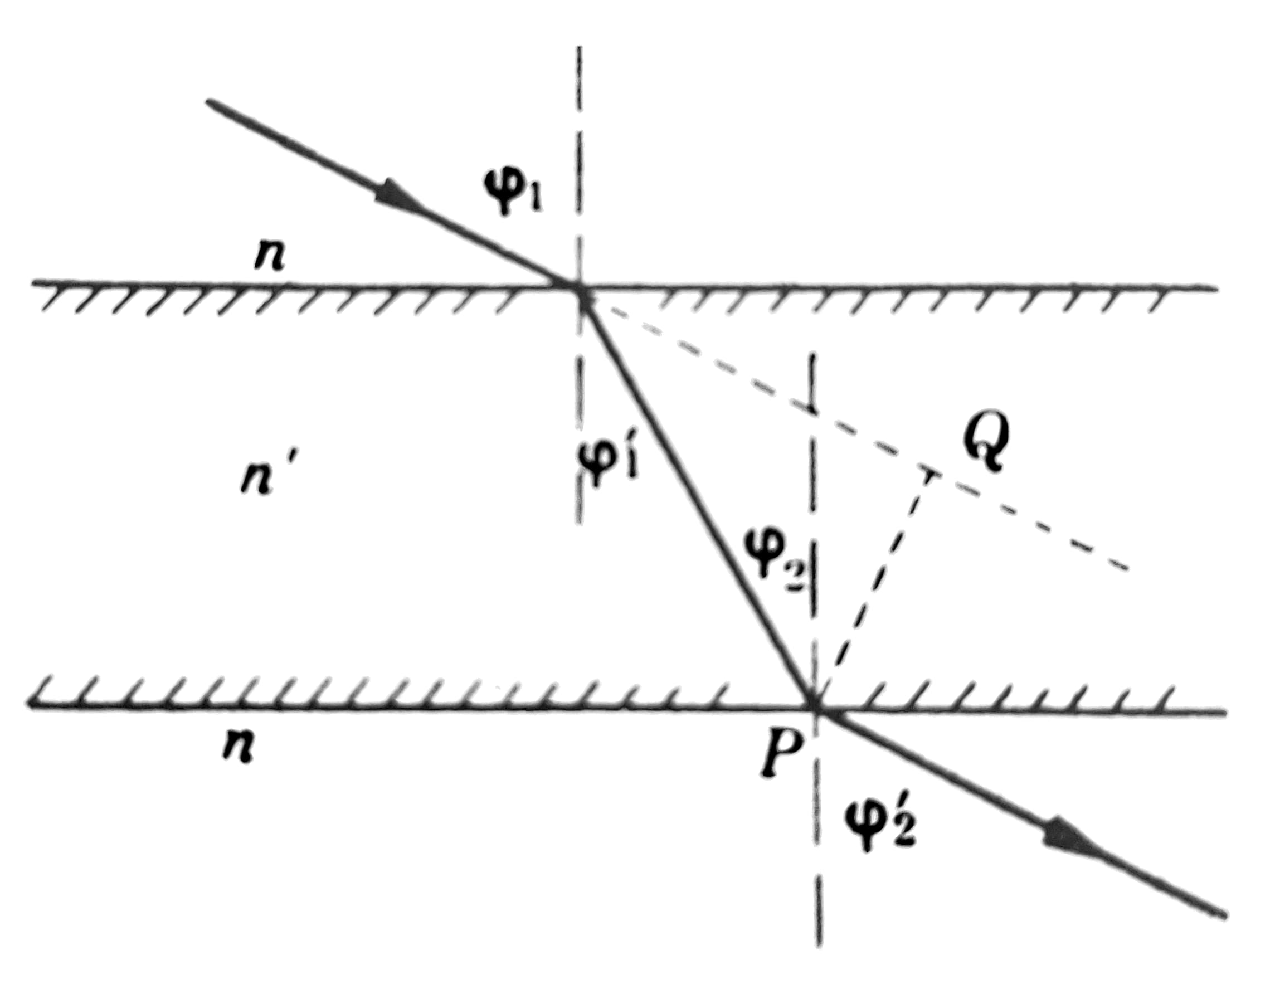
\includegraphics[width=\textwidth]{../../figs/lamina caras paralelas.pdf}
            \caption{Esquema del Ejercicio~\ref{ej:laminas_paralelas}.}
            \label{fig:lamina_paralelas}
        \end{subfigure}
        \caption{}
    \end{figure}

    \pagebreak

    \question Una onda electromagnética plana y monocromática que se propaga a lo largo del eje $x$, es emitida por una fuente que se encuentra en $+\infty$ e incide sobre una superficie plana perfectamente conductora ubicada en el plano $yz$, es decir $x=0$.
    \begin{parts}
        \part Hallar la expresión del campo eléctrico ($\vec{E}_i$) y del campo magnético ($\vec{B}_i$) correspondientes a la onda electromagnética plana monocromática que incide sobre la superficie conductora, teniendo en cuenta que la polarización del campo eléctrico es paralela a $\ver{e}_y$.
        \part Si la condición de contorno correspondiente a la superficie conductora exige que la componente del campo eléctrico total que es tangencial a la misma debe anularse cuando la onda llega a esta a dicha superficie para todo $y$, $z$ y $t$, mostrar que las expresiones de $\vec{E}$ y de $\vec{B}$ (campos totales) que satisfacen la condición de contorno son $$ \vec{E} \left(x,t\right) = -\, 2 \, E_{0,i} \sen \left(\omega \, t\right) \sen \left(k \, x\right) \, \ver{e}_y \qquad \text{ y } \qquad \vec{B} \left(x,t\right) = - \, \frac{2 \, E_{0,i}}{c} \cos \left(\omega \, t\right) \cos \left(k \, x\right) \, \ver{e}_z, $$ donde $E_{0,i}$ es la amplitud del campo eléctrico incidente, $\omega$ es la frecuencia angular, $k$ es el número de onda.
        \part Mostrar que si se agrega otra superficie perfectamente conductora en el $x=L$, paralela a la anterior, entonces las ondas electromagnéticas que pueden propagarse confinadas entre $0$ y $L$ solamente pueden tener frecuencias bien definidas.
    \end{parts}

    \question Dos cuerdas de densidades $\rho_1$ y $\rho_2$ están unidas en $x=0$, están sometidas a la misma tensión y sus respectivas secciones transversales tienen áreas iguales. Si $y_1 (x,t) = f_1 \left(x - v_1 \, t\right)$ representa una onda que incide en $x=0$ desde $-\infty$, a partir del análisis de la discontinuidad se obtiene que debe haber, en general, una onda reflejada $g_1$ y una onda transmitida $f_2$, las cuales pueden determinarse mediante las expresiones: $$ g_1 \left(x + v_1 \, t\right) = C_R \, f_1 \left(x + v_1 \, t\right) \qquad \text{ y } \qquad f_2 \left(x - v_2 \, t\right) = C_T \, f_1 \left(x - v_2 \, t\right), $$ donde $$ C_R = \frac{v_2 - v_1}{v_2 + v_1} \qquad \text{ y } \qquad C_T = \frac{2 \, v_2}{v_2 + v_1} $$ son los llamados coeficientes de reflexión y de transmisión, respectivamente. Considerando las posibles relaciones entre las densidades de las cuerdas, demostrar que $-1 \le C_R \le 1$ y que $0 \le C_T \le 2$, por lo que, en consecuencia, $C_T - C_R = 1$.

    \question Enunciar el principio de Huygens y, a partir de este, deducir la ley de la reflexión y la ley de Snell. Para ello, considere una onda plana monocromática que incide sobre una superficie plana, con un cierto ángulo de incidencia $\varphi_i$, medido respecto de la dirección perpendicular al plano sobre el que incide la onda. Además, considerar que esta superficie divide dos medios, uno de índice de refracción $n$, en donde se propaga la onda incidente y la reflejada, y otro de índice de refracción $n'$, en donde se propaga la onda refractada.

    \question Enunciar el principio de Fermat y describir cómo se podrían obtener las leyes de la reflexión y de la refracción usando este principio.

    \question Un haz de luz incide bajo un ángulo $\varphi_1$ sobre la superficie superior de una lámina transparente cuyas superficies son planas y paralelas entre sí, tal como se muestra en la Figura~\ref{fig:lamina_paralelas}. \label{ej:laminas_paralelas}
    \begin{parts}
        \part Demostrar que $\varphi_1 = \varphi_2'$.
        \part Demostrar que esto se verifica se verifica para un número láminas paralelas diferentes.
        \part Demostrar que el desplazamiento lateral $d$ del haz emergente (distancia entre los puntos $P$ y $Q$) viene dado por la relación: $$ d = h \frac{\sen \left(\varphi_1 - \varphi_1'\right)}{\cos \varphi_1'}, $$ donde $h$ es el ancho de la lámina, esto es, la distancia entre sus caras.
    \end{parts}

    \question Dos orificios separados por $0.5$ mm están iluminados por un haz de láser helio-neón que emite luz monocromática de longitud de onda de $0.6328 \E{-6}$ m. Una pantalla está ubicada 5 m detrás de aquella que contiene a los orificios. 
    \begin{parts}
        \part ¿Cuál es la separación de las franjas de interferencia sobre la pantalla?
        \part ¿A qué se debe la diferencia de fases entre las ondas emitidas desde los orificios que producen las franjas oscuras y brillantes, típicas del patrón de interferencia en este caso? ¿Cuáles son las hipótesis bajo las cuales se obtiene la expresión que permite calcular la separación de las franjas?
    \end{parts}

\end{questions}

\end{document}